\documentclass[english]{scrartcl}
\usepackage[T1]{fontenc}
\usepackage[utf8]{inputenc}
\usepackage{lmodern}
\usepackage{graphicx}
\usepackage{babel,blindtext}
\usepackage{float}
\usepackage{wrapfig}	
%opening
\title{PH21 Assignment 4 Report     updated last section}
\author{Helen Xue}

\begin{document}

\maketitle

\section{Coin}
\par true probability H = 0.4:
\begin{figure}[H]
	\minipage{0.32\textwidth}
	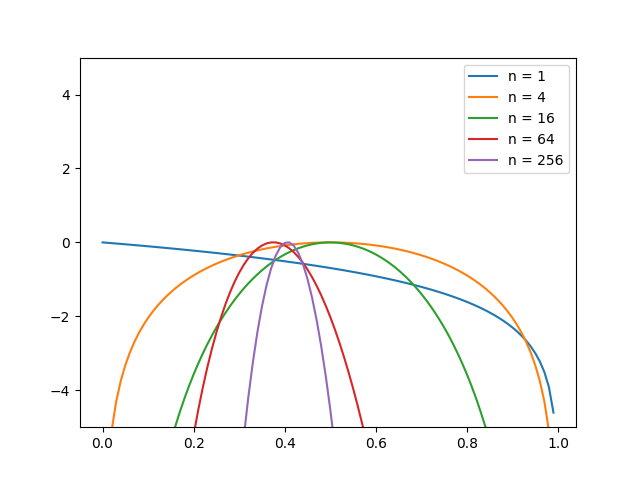
\includegraphics[width=\linewidth]{coin/h=0.4/gauss_1sigma}
	\caption{gauss, within 1 sigma}  
	\endminipage \hfill
	\minipage{0.32\textwidth}
	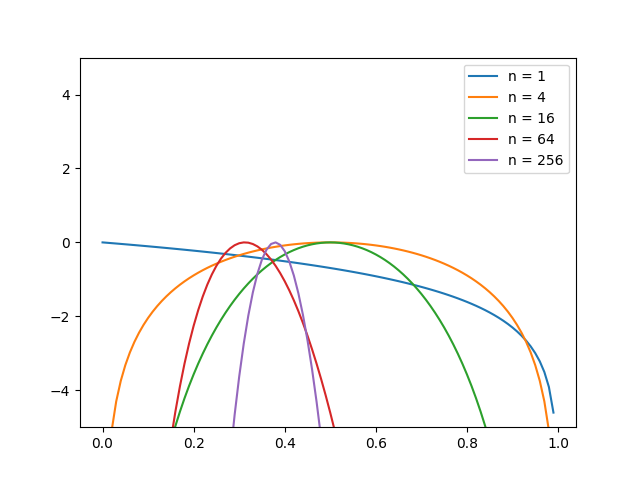
\includegraphics[width=\linewidth]{coin/h=0.4/gauss_3sigma}
	\caption{gauss, within 3 sigma} 
	\endminipage \hfill
		\minipage{0.32\textwidth}
	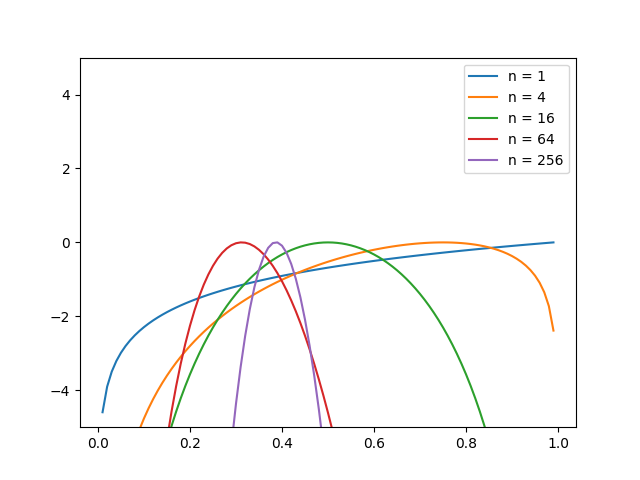
\includegraphics[width=\linewidth]{coin/h=0.4/gauss_far}
	\caption{gauss, very far from true value} 
	\endminipage \hfill
		\minipage{0.32\textwidth}
	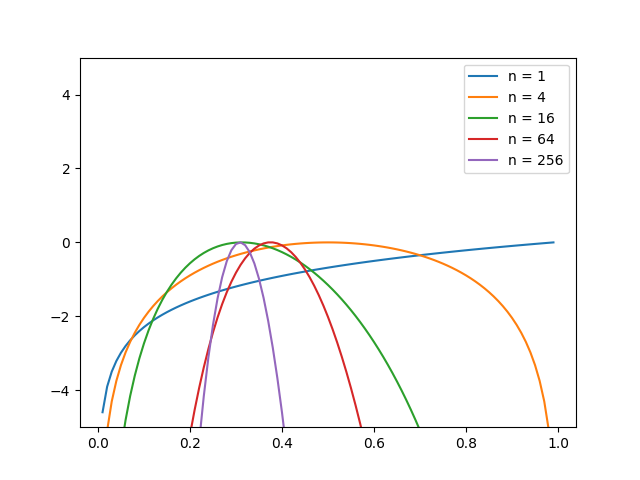
\includegraphics[width=\linewidth]{coin/h=0.4/unif}
	\caption{uniform} 
	\endminipage \hfill
\end{figure}

\par We can see that the closer the prior is to the true value, the tighter the peaks are. As the number of trials increase, we get closer to the true value, which is what we would expect.
\par The curves for $n=1$ and $n=2$ are always haphazard, since there are so few trials. 
\newpage
\par true probability H = 0.8:
\begin{figure}[H]
	\minipage{0.32\textwidth}
	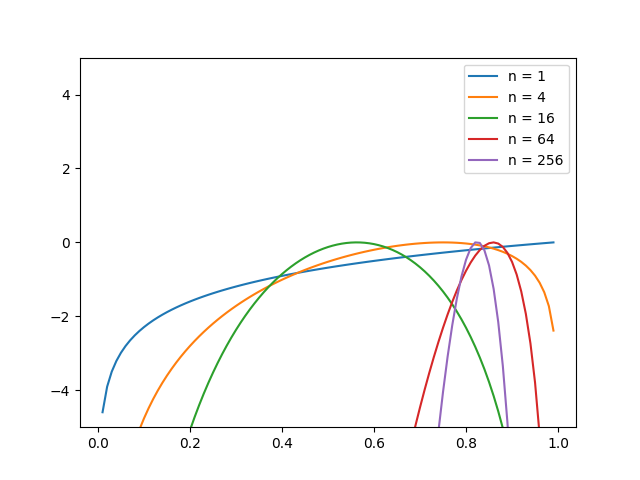
\includegraphics[width=\linewidth]{coin/h=0.8/gauss_1sigma}
	\caption{gauss, within 1 sigma}  
	\endminipage \hfill
	\minipage{0.32\textwidth}
	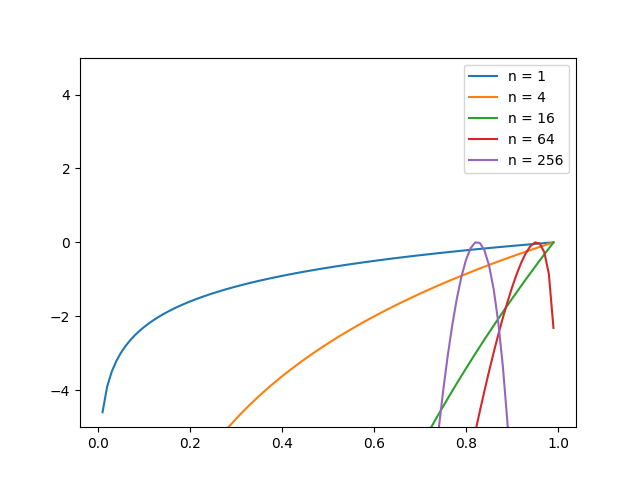
\includegraphics[width=\linewidth]{coin/h=0.8/gauss_3sigma}
	\caption{gauss, within 3 sigma} 
	\endminipage \hfill
	\minipage{0.32\textwidth}
	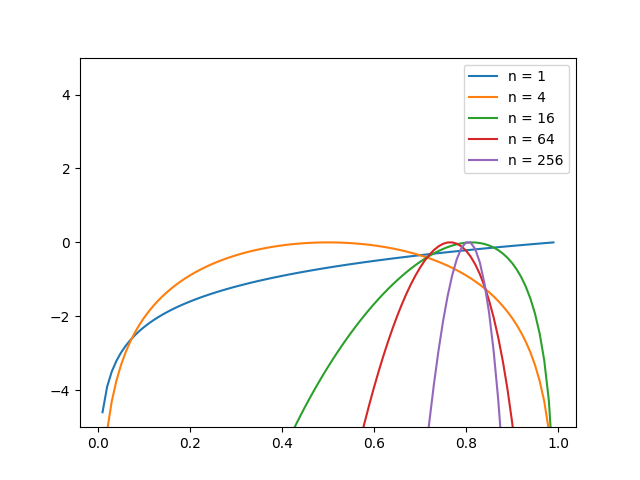
\includegraphics[width=\linewidth]{coin/h=0.8/gauss_far}
	\caption{gauss, very far from true value} 
	\endminipage \hfill
	\minipage{0.32\textwidth}
	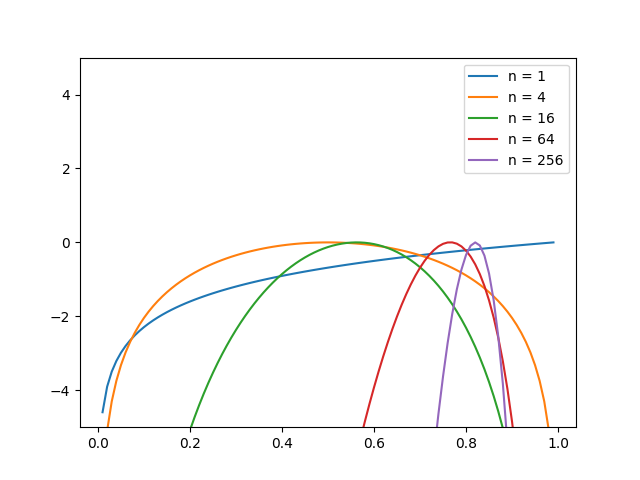
\includegraphics[width=\linewidth]{coin/h=0.8/unif}
	\caption{uniform} 
	\endminipage \hfill
\end{figure}

\par We can clearly see that the peak-cluster-center has been shifted over to 0.8, especially for the larger trial numbers.

\section{Lighthouse: beta known}
\par We can use trigonometric relations to find the number of hits, as depending on alpha and beta.
\par Letting our random variable $\theta$ be randomly and uniformly distributed, we count a flash as a hit h if in $n$ values of $\theta$, any $\theta_n$ is between $\frac{\pi}{2}$ and $\frac{3\pi}{2}$. 
\par The location where a successful flash is received is then $btan(\theta)+a$.
\par Using this and a prior for a, we get results as follows:
\newpage
\par true alpha = 1.0
\begin{figure}[H]
	\minipage{0.32\textwidth}
	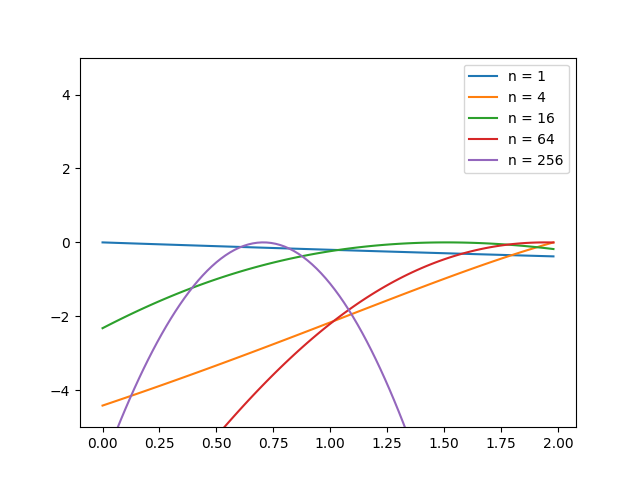
\includegraphics[width=\linewidth]{lighthouse/1d/h=0.4/gauss_1sigma}
	\caption{gauss, within 1 sigma}  
	\endminipage \hfill
	\minipage{0.32\textwidth}
	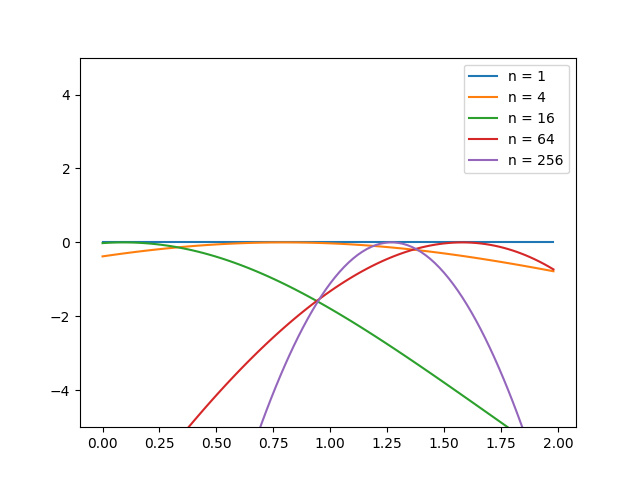
\includegraphics[width=\linewidth]{lighthouse/1d/h=0.4/gauss_3sigma}
	\caption{gauss, within 3 sigma} 
	\endminipage \hfill
	\minipage{0.32\textwidth}
	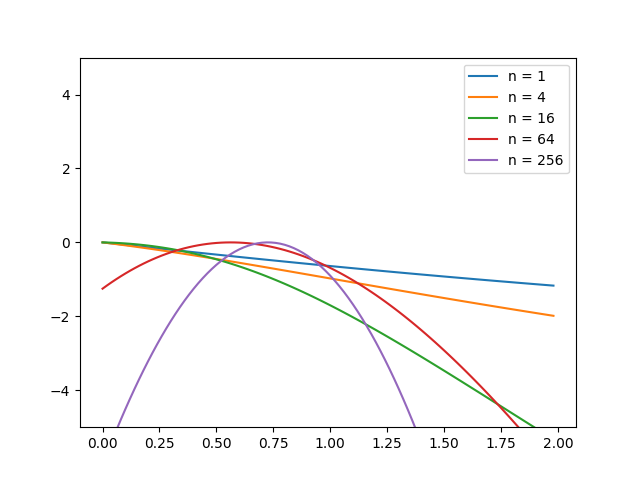
\includegraphics[width=\linewidth]{lighthouse/1d/h=0.4/gauss_far}
	\caption{gauss, very far from true value} 
	\endminipage \hfill
	\minipage{0.32\textwidth}
	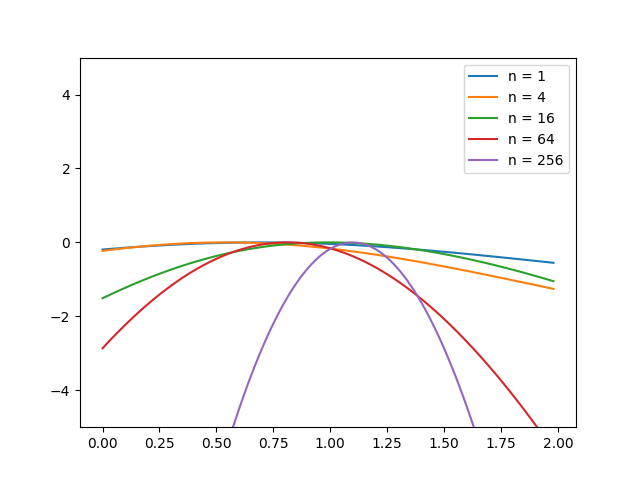
\includegraphics[width=\linewidth]{lighthouse/1d/h=0.4/unif}
	\caption{uniform} 
	\endminipage \hfill
\end{figure}

\par This time, with a more complicated situation, the true value is much harder to pin down with the same number of trials. The peaks are generally much wider; we still see them narrow as n increases.

\par The mean is not a good estimator since the Central Limit Theorem doesn't apply to Cauchy distributions.

\newpage
\section{Lighthouse, neither alpha nor beta known: updated}
\par When we know neither a nor b, we can still use this technique to generate a heatmap of likelihoods by using the same prior twice for a and b; here $a=1.0$, $b=1.5$, and a is on the x axis, and b is on the y axis.

\par Results for different n:
\par n=4
\begin{figure}[H]
	\minipage{0.32\textwidth}
	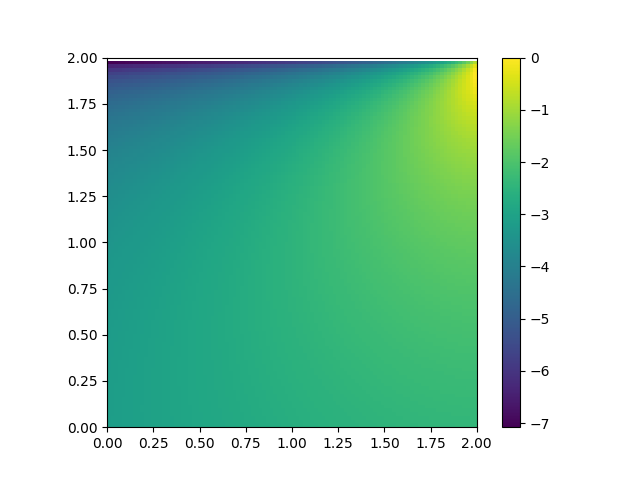
\includegraphics[width=\linewidth]{lighthouse/2d/gauss_1sigma_n=4}
	\caption{gauss, within 1 sigma}  
	\endminipage \hfill
	\minipage{0.32\textwidth}
	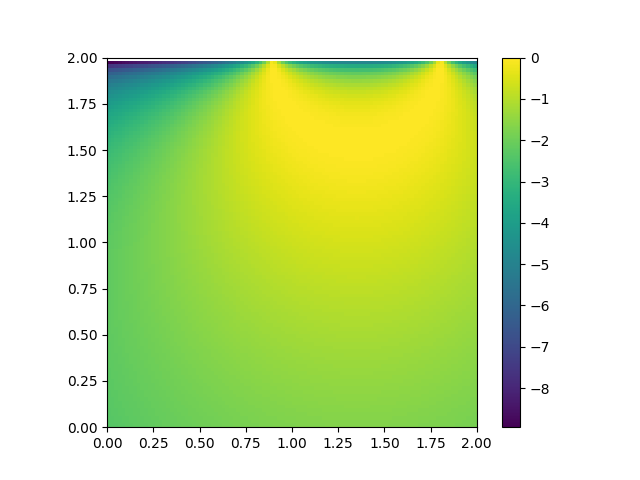
\includegraphics[width=\linewidth]{lighthouse/2d/gauss_3sigma_n=4}
	\caption{gauss, within 3 sigma} 
	\endminipage \hfill
	\minipage{0.32\textwidth}
	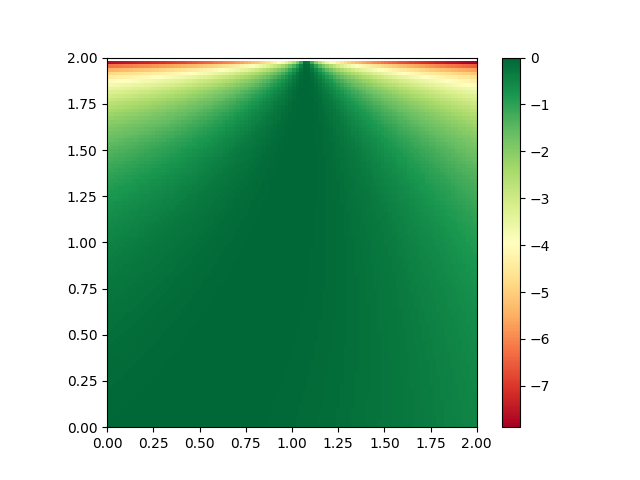
\includegraphics[width=\linewidth]{lighthouse/2d/unif_n=4}
	\caption{uniform} 
	\endminipage \hfill
\end{figure}

\par n=16
\begin{figure}[H]
	\minipage{0.32\textwidth}
	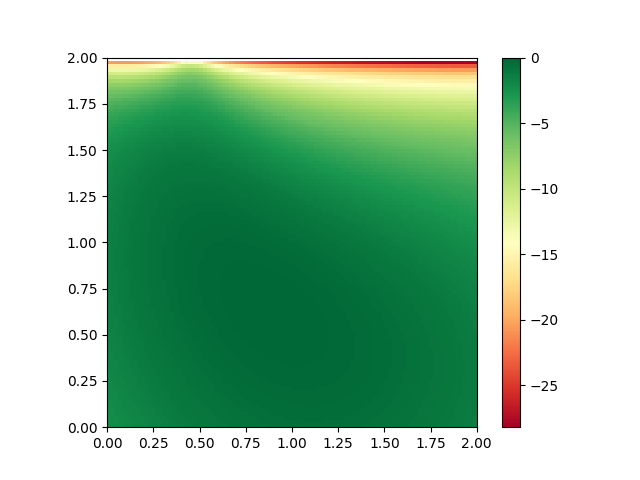
\includegraphics[width=\linewidth]{lighthouse/2d/gauss_1sigma_n=16}
	\caption{gauss, within 1 sigma}  
	\endminipage \hfill
	\minipage{0.32\textwidth}
	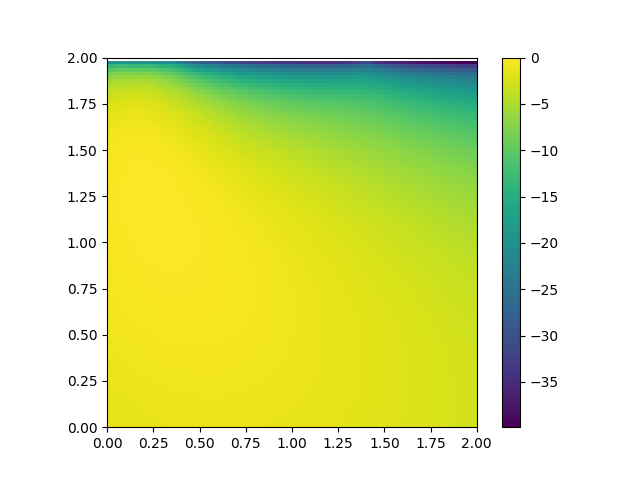
\includegraphics[width=\linewidth]{lighthouse/2d/gauss_3sigma_n=16}
	\caption{gauss, within 3 sigma} 
	\endminipage \hfill
	\minipage{0.32\textwidth}
	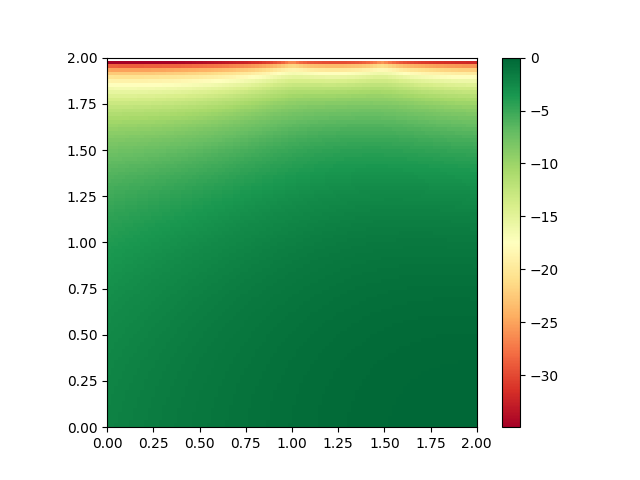
\includegraphics[width=\linewidth]{lighthouse/2d/unif_n=16}
	\caption{uniform} 
	\endminipage \hfill
\end{figure}

\par n=64
\begin{figure}[H]
	\minipage{0.32\textwidth}
	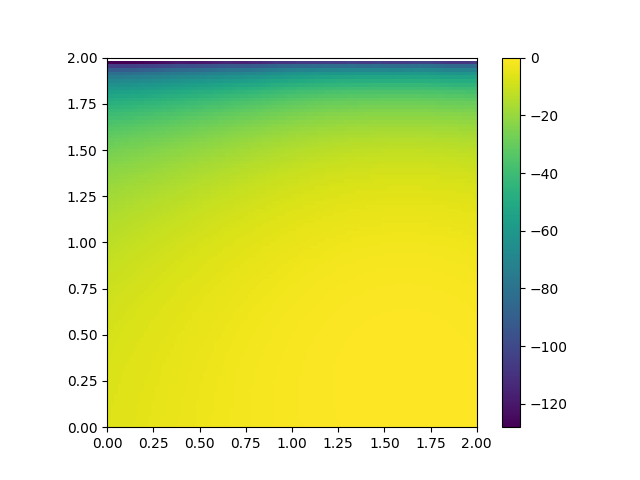
\includegraphics[width=\linewidth]{lighthouse/2d/gauss_1sigma_n=64}
	\caption{gauss, within 1 sigma}  
	\endminipage \hfill
	\minipage{0.32\textwidth}
	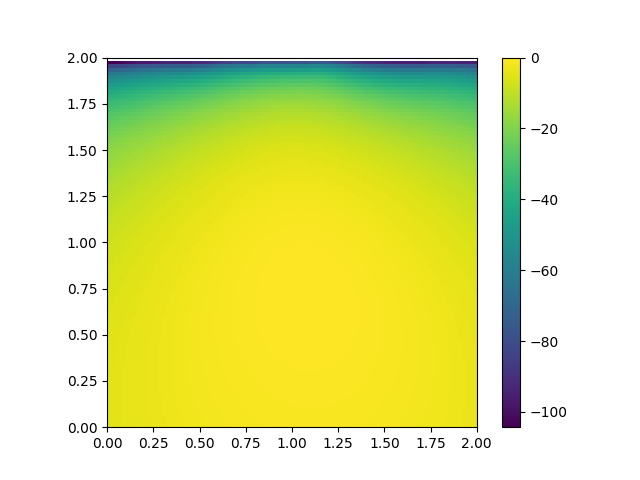
\includegraphics[width=\linewidth]{lighthouse/2d/gauss_3sigma_n=64}
	\caption{gauss, within 3 sigma} 
	\endminipage \hfill
	\minipage{0.32\textwidth}
	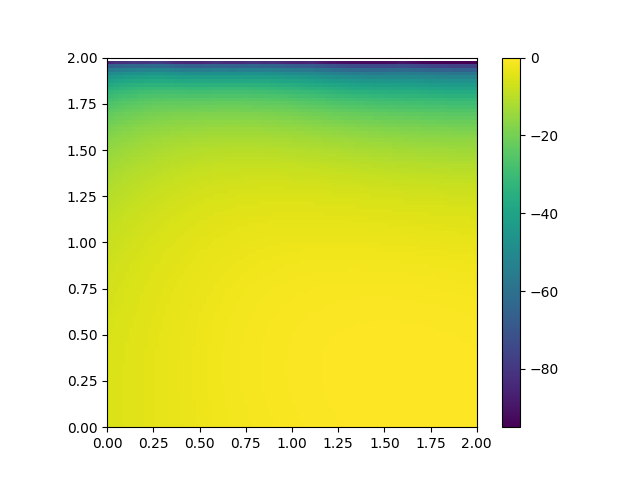
\includegraphics[width=\linewidth]{lighthouse/2d/unif_n=64}
	\caption{uniform} 
	\endminipage \hfill
\end{figure}

\par n=256
\begin{figure}[H]
	\minipage{0.32\textwidth}
	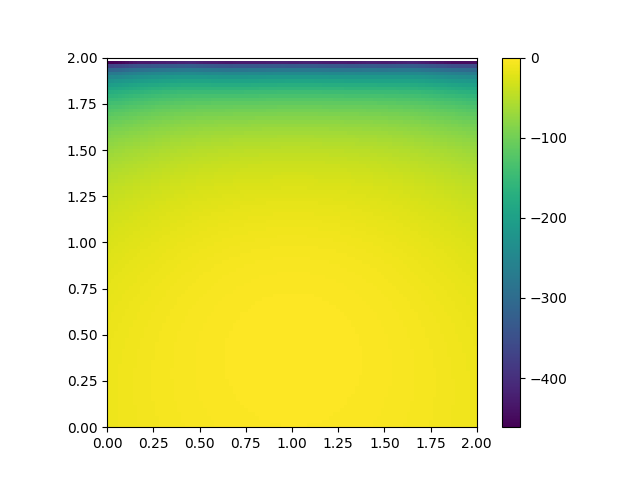
\includegraphics[width=\linewidth]{lighthouse/2d/gauss_1sigma_n=256}
	\caption{gauss, within 1 sigma}  
	\endminipage \hfill
	\minipage{0.32\textwidth}
	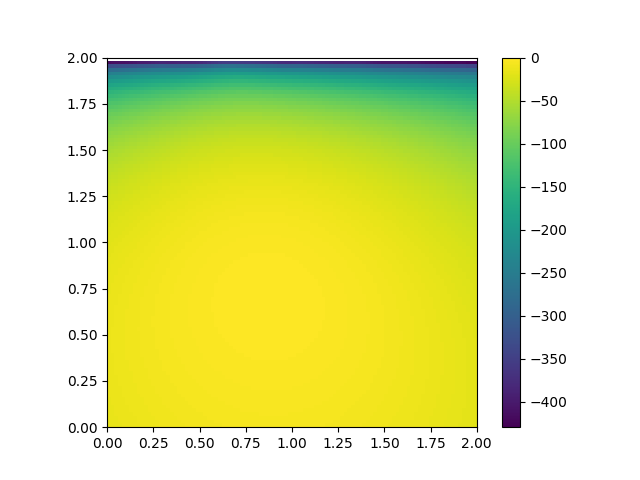
\includegraphics[width=\linewidth]{lighthouse/2d/gauss_3sigma_n=256}
	\caption{gauss, within 3 sigma} 
	\endminipage \hfill
	\minipage{0.32\textwidth}
	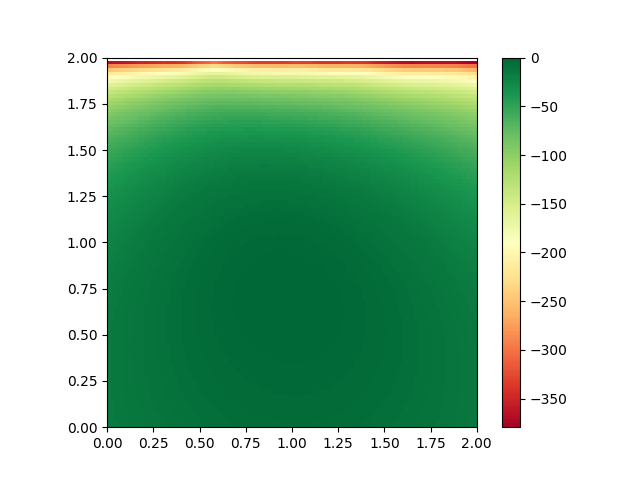
\includegraphics[width=\linewidth]{lighthouse/2d/unif_n=256}
	\caption{uniform} 
	\endminipage \hfill
\end{figure}


\par Updates: Previously, I'd only included one prior in the calculation instead of both. After fixing that and changing the extent of the plot to better bracket the data, we can see that the tight gaussian prior has narrow peaks (rings), and as we increase the sample size, the peak approaches our true $(alpha,beta)$ location.
\par The wider gaussian did better than the uniform, but both look too broad to be very useful.

\end{document}
